\newthought{A \index{complex sinusoidal signal}{complex sinusoidal signal} is the elementary building block of the Fourier decomposition of a signal}. 
This signal is fully determined by three parameters:\index{amplitude}{amplitude} $A \in \mathbb{R}_{\ge 0}$, \index{phase}{phase} $\phi \in \mathbb{R}$ (rad), and
\index{angular frequency}{angular frequency} $\omega \in \mathbb{R}$ (rad/s).
\begin{equation}
\boxed{
z(t) = A e^{i(\omega t + \phi)} = A e^{i\phi} e^{i\omega t} = X e^{i\omega t}.
}
\end{equation}
It is possible to combine phase and amplitude as one complex constant $X = Ae^{i\phi} \in \mathbb{C}$. This constant contains information about the amplitude and phase of the signal. $X$ is often referred to as a \emph{\index{phasor}{phasor}}.

\begin{marginfigure}
\begin{center}
\begin{tikzpicture}
	\begin{axis}[domain=0:(2*6.23),
        width=7cm,
        height=7cm,
        ticks=none,
        axis lines = center,
        ymax=2,
        ymin=-2,
        samples=200,
        legend pos=north east,
        legend style={draw=none},
        xlabel={$t$},
        ylabel={$e^{i\omega t}$}]
    \addplot[blue] {cos(2*deg(x))};
    \addplot[red] {sin(2*deg(x))};

    \node at (axis cs:3.14,-1.5) {$\displaystyle{T=\frac{2\pi}{\omega}}$};   
    \addplot [dimen] plot coordinates {(1.57,-1.1) (4.71,-1.1)};
    
    \legend{$\mathrm{Re}(e^{i\omega t})$,$\mathrm{Im}(e^{i\omega t})$}
    \end{axis}
\end{tikzpicture}
\end{center}
\caption{A complex sinusoidal signal is the basic building block (basis function) in a Fourier decomposition of a signal. The fundamental period $T=2\pi/\omega$
of this signal is also shown.}
\label{fig:complex_sinusoid}
\end{marginfigure}

\begin{marginfigure}
\begin{center}
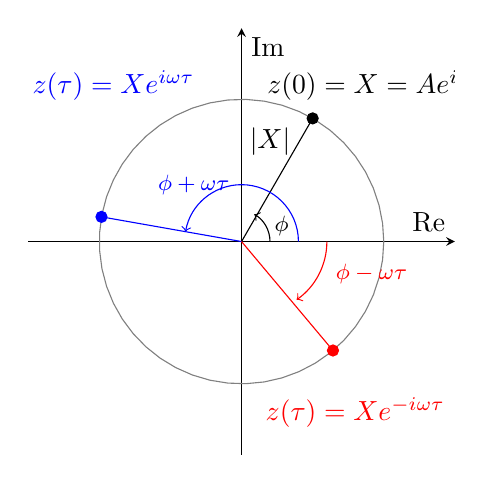
\begin{tikzpicture}
	\begin{axis}[axis equal, disabledatascaling,
    ymin=-1.5,xmin=-1.5,ymax=1.5,xmax=1.5, ticks=none,
    xlabel=$\mathrm{Re}$, ylabel=$\mathrm{Im}$, axis lines = center,
    width=7cm, height=7cm] \addplot
    [gray,domain=0:2*pi,samples=50]({cos(deg(x))},{sin(deg(x))});
    
    \addplot [black, mark = *] coordinates {( {cos(60)}, {sin(60)} )} {};   
     \addplot [black] coordinates { (0,0) ( {cos(60)}, {sin(60)} ) };

    \addplot [blue, mark = *] coordinates {( {cos(170)}, {sin(170)} )} {};   
     \addplot [blue] coordinates { (0,0) ( {cos(170)}, {sin(170)} ) };

   \addplot [red, mark = *] coordinates {( {cos(-50)}, {sin(-50)} )} {};   
     \addplot [red] coordinates { (0,0) ( {cos(-50)}, {sin(-50)} ) };

  \draw[draw=black, ->] (axis cs:0.2,0) arc [radius=0.4cm,start angle=0,end angle=60]
  node[midway,right,inner sep=3pt,font={\footnotesize}]{$\phi$};

%  \draw[draw=blue] (axis cs:1,0) arc [radius=0.5cm,start angle=60,end angle=120]
%  
\draw [blue, ->] (axis cs:0.4,0.0) arc [radius=0.4,start angle=0,end angle=170]
node[midway,left,inner sep=6pt,font={\footnotesize}]{$\phi+\omega \tau$};

\draw [red, ->] (axis cs:0.6,0.0) arc [radius=0.5,start angle=0,end angle=-55]
node[midway,right,inner sep=6pt,font={\footnotesize}]{$\phi-\omega \tau$};

 \node at (axis cs:0.9,1.1) {$z(0)=X=Ae^{i\phi}$};

 \node at (axis cs:0.2,0.7) {$|X|$};

 \node[blue] at (axis cs:-0.9,1.1) {$z(\tau)=X e^{i\omega \tau}$};
 \node[red] at (axis cs:0.8,-1.2) {$z(\tau)=X e^{-i\omega \tau}$};
\end{axis}
\end{tikzpicture}
\end{center}
\caption{A complex sinusoidal signal on the complex plane can be seen as a point moving around a circle. For positive frequencies, the point rotates around the circle in counterclockwise direction. For negative frequencies, the rotation is clockwise.}
\label{fig:rotating_phasor}
\end{marginfigure}

Using Euler's formula, we can express the \index{complex sinusoidal signal}{complex sinusoidal signal} as a function of \index{$\cos$}{$\cos$} and \index{$\sin$}{$\sin$}:
\begin{equation}
Ae^{i(\omega t + \phi)}= A[\cos(\omega t + \phi) + i \sin(\omega t + \phi)].
\end{equation}
With this formulation, it is apparent that the real and imaginary components are identical sinusoidal signals, which are 90 degrees out of phase with each other, because we know that $\cos(\theta)
= \sin(\theta + \pi/2)$. Figure \ref{fig:complex_sinusoid} shows an example of a complex sinusoidal signal.

You can also think of a complex sinusoidal signal as a point on the complex plane, which rotates around in a circle around the origin. This is sometimes referred to as the \emph{rotating phasor}. The radius of the circle is the amplitude of the signal $A=|X|$. At $t=0$, the point is at a phase angle of $\phi$. This phase angle as a function of time is given by $\phi + \omega t$ and determines the position of the point on the circle at a given time. If $\omega>0$, then the point moves counterclockwise around the circle when the value of $t$ increases. If $\omega < 0$, then the point moves
in the clockwise direction around the circle as the value of $t$ increases. Figure \ref{fig:rotating_phasor} depicts this concept.

This might at first seem like an unnecessarily complicated way to express a sinusoidal signal, but this representation often simplifies the mathematics. For example, it is in most cases much easier to algebraically work with the function $\frac{1}{2}(e^{i\phi}e^{i\omega
t}+e^{-i\phi}e^{-i\omega t})$ than it is with $\cos(\omega t + \phi)$, even though they are the same thing.

You'll also see, later on, that a complex sinusoidal signal is
an \emph{\index{eigenfunction}{eigenfunction}} for any linear
time-invariant operator. It allows us to characterize the properties of a linear time-invariant system just by simply investigating what effect the system has on a complex sinusoidal signal. If we spend the effort to learn how to use a complex sinusoidal signal, then we'll know everything there is to know about linear time-invariant systems!

\newthought{Real valued sinusoidal signals can be related to complex sinusoidal signals}. Using the inverse Euler relationship, we can express a real valued sinusoidal signal of some amplitude, angular frequency, and phase. By taking the real or imaginary part of a complex sinusoidal signal, we obtain a cosine or sine signal.

Using the earlier definition of a complex sinusoidal signal, we find that:
\begin{align}
\Re{z(t)} &= \frac{1}{2}\left[X e^{i\omega t} + X^* e^{-i\omega t}\right] = A\cos(\omega t + \phi) \label{eq:resignal} \\
\Im{z(t)} &= \frac{1}{2i}\left[X e^{i\omega t} - X^* e^{-i\omega t}\right] = A\sin(\omega t + \phi) \label{eq:imsignal}
\end{align}
This tells us that a real valued sinusoidal signal with angular frequency $\omega$ is a sum of a positive and negative frequency complex sinusoidal signal with angular frequencies $\pm\omega$. Note that the sign of the phase angles of the two complex sinusoidal signals are also $\pm\phi$.

\newthought{Angular frequency $\omega$} of a complex sinusoidal signal, determines how many radians the phase of the signal advances per unit of time. If the unit of time is seconds, the angular frequency has units of \emph{radians per second} (rad/s).

It is possible to relate angular frequency to frequency $f$ in units of cycles per time unit, i.e., how many times does the point whose position is indicated by the complex sinusoidal signal rotate around the circle per unit of time:
\begin{equation}
\boxed{\omega = 2\pi f}
\end{equation}
If the unit of time is seconds, then the unit of frequency $f$ is hertz (Hz or 1/s). Sometimes \emph{cycles per second} is indicated as the unit for frequency. 

I will try to consistently use the name \emph{angular frequency} and symbol $\omega$ when referring to a frequency that is in units of radians per unit of $t$. I will use the name \emph{\index{frequency}{frequency}} and the symbol $f$ when referring to the frequency that is in units of cycles
per unit of $t$. In some cases, when I am talking about frequency in general, and it does not matter what the units are, I will drop the word angular and just talk about frequency.

It is unfortunate that these two competing units exist. 
It occasionally causes confusion even for people who have worked with signals for many years! 
It is not unusual to find a factor of $2\pi$ missing or unnecessarily added in a textbook that is discussing the frequency of a signal.

Throughout these lecture notes, we will most of the time call the independent variable $t$ of a one dimensional signal time and assign it units of seconds. 
However, the physical units of $t$ do not necessarily have to be seconds, and $t$ does not have to denote time.

For example, if the units of $t$ were distance in meters, then we would have an angular frequency $\omega$ that is in units of radians per meter, and frequency $f$ that is in units of cycles per meter. In physics, a spatial frequency is typically called a \emph{\index{wavenumber}{wavenumber}}. It is customary to use the symbol $k$ for angular wavenumber and the Greek letter $\nu$ for linear wavenumber. These types of spatial frequencies are often encountered when dealing with propagating waves. There is an example at the end of this chapter on this topic.

\newthought{Complex and real valued sinusoidal signals} are periodic. The definition of a \index{periodic function}{periodic function} requires that the function repeats after a certain time period $T$ for all values of $t$:
\begin{equation}
\boxed{z(t) = z(t+ n T).}
\end{equation}
where $n \in \mathbb{Z}$ and $T \in \mathbb{R}_{>0}$.  

The smallest possible positive non-zero value of $T$ is called the \emph{\index{fundamental period}{fundamental period}} of the function. 

In the case of complex sinusoidal signals, the definition of periodicity yields:
\begin{align}
Ae^{i (\omega t + \phi)}= Ae^{i (\omega (t+T) + \phi)} = Ae^{i (\omega t+ \omega T + \phi)}
\end{align}
By definition, we know that a complex sinusoidal signal is
$2\pi$-periodic, in other words
\begin{equation}
Ae^{i\theta}=Ae^{i(\theta+2\pi k)}
\end{equation}
for $k\in\mathbb{Z}$. By setting $\theta = \omega t +\phi$, this implies that $\omega T = 2\pi k$.

In order to look for the smallest value of $T$, we inspect the case where $k=1$, from which it follows that the fundamental period is:
\begin{equation}
\boxed{T = \frac{2\pi}{\omega} = \frac{1}{f}.}
\end{equation}
The fundamental period for a complex sinusoidal signal is shown in Figure \ref{fig:complex_sinusoid}.

\newthought{Multiple complex sinusoidal signals with the same frequency but possibly different phases and amplitudes can be added together to form one complex sinusoidal signal}. This is sometimes referred to as the \emph{\index{phasor summation}{phasor summation}}\sidenote{The signal $A e^{i\phi}e^{i\omega t}$ is called a phasor if $A$, $\phi$, and $\omega$ have no time dependence.} property.

Let us assume that we have $N$ complex sinusoidal signals. Each one of these signals has the same angular frequency $\omega$ but different phases $\phi_n$ and amplitudes $A_n$. If we add these together, we get one complex sinusoidal signal with an amplitude $A$ and phase $\phi$:
\begin{equation}
\sum_{n=1}^N A_n e^{i(\omega t + \phi_n)} = A e^{i (\omega t + \phi)}
\end{equation}
This is relatively easy to see. Let's define $X_n = A_n e^{i\phi_n}$, which allows us to rewrite the sum in the following form:
\begin{align}
\sum_{n=1}^N A_n e^{i(\omega t + \phi_n)} &= \sum_{n=1}^N X_n e^{i\omega t} \\
&= \underbrace{\left(\sum_{n=1}^N X_n\right)}_{X} e^{i\omega t} \\
&= X e^{i\omega t}\\
&= |X| e^{i\angle X} e^{i\omega t}\\
&= A e^{i \phi} e^{i\omega t}
\label{eq:sum_sinusoids}
\end{align}
Here $X=\sum_n X_n$ is just a sum of constant valued complex numbers that contain information about the phases and amplitudes of the individual complex sinusoids.

\newthought{Multiplying two complex sinusoidal signals together is equivalent to a shift in frequency and phase}.
Consider two complex sinusoidal signals with angular frequencies $\omega_1$ and $\omega_2$, and phase angles $\phi_1$ and $\phi_2$. For the sake of simplicity, we'll assume that both signals are unit amplitude:
\begin{align}
z_1(t) &=  e^{i(\omega_1 t + \phi_1)}\\
z_2(t) &=  e^{i(\omega_2 t + \phi_2)}
\end{align}
Multiplying together these two signals $z_3(t) = z_1(t)z_2(t)$ we get:
\begin{equation}
\boxed{e^{i(\omega_3 t + \phi_3)}  = e^{i[(\omega_1 + \omega_2) t + (\phi_1+\phi_2)]}}
\label{eq:freqmix}
\end{equation}
The resulting signal $z_3(t)$ is a complex sinusoid, at a new frequency: $\omega_3 = \omega_1 + \omega_2$ and phase $\phi_3=\phi_1+\phi_2$.

This property is one of the elementary operations in signal
processing. For example, we'll use multiplication of two complex sinusoidals signals later on as part of the proof of the Shannon-Nyquist sampling theorem.

The frequency shift property is also widely used in radio engineering and telecommunications to shift high frequency signals to lower frequencies and vice versa. This operation is called downconversion or upconversion in radio engineering terminology.

\newthought{It is possible to extend the concept of a complex sinusoidal signal into multiple dimensions}. For example, a \index{two dimensional complex sinusoidal
signal}{two-dimensional complex sinusoidal
signal} would be of the form:
\begin{equation}
z(x,y) = A e^{i\phi} e^{i k x} e^{i \ell y}.
\end{equation}
Here $k$ and $\ell$ are the angular frequencies in the $x$ and $y$ directions.

In the last example\sidenote{I couldn't resist using this nice example, even though this course is about 1d signals.} of this chapter, we'll show how to use a two-dimensional complex sinusoidal signal to derive the plane wave solution of electromagnetic waves propagating in free space from Maxwell's equations.

\newthought{A time-shift is equivalent to a phase shift for a complex sinusoidal signal}.
Let's investigate a time-shift system, which shifts time by a constant $\tau$:
\begin{equation}
y(t) = \mathcal{T}\{x(t)\} = x(t-\tau),
\end{equation}
which means that the output signal at time $t$ is the same as the input signal at time $t-\tau$. One could also say that the output signal is delayed by a time constant $\tau$.

\pgfplotsset{
    dirac/.style={
        mark=triangle*,
        mark options={scale=2},
        ycomb,
        scatter,
        visualization depends on={y/abs(y)-1 \as \sign},
        scatter/@pre marker code/.code={\scope[rotate=90*\sign,yshift=-2pt]}
    }
}
\begin{marginfigure}[-2cm]
\begin{center}
\begin{tikzpicture}
\begin{axis}[width=7cm,height=4cm,ymin=0,xmin=-0.5,ymax=1.1,xmax=1.5,         
        yticklabels={,,},
        xtick={0,1},
        xticklabels={$0$,$\tau$},
        xlabel=$t$,
        axis y line=middle, axis x line=bottom] 
%        , axis lines = center]
\addplot +[dirac,blue] coordinates {(1,1)};
\node at (axis cs:0.75,1) [below, blue, font={\footnotesize}]{$\delta(t-\tau)$};
\addplot +[dirac,red] coordinates {(0,1)};
\node at (axis cs:-0.15,1) [below, red, font={\footnotesize}]{$\delta(t)$};
\end{axis}
\end{tikzpicture}
\end{center}
\caption{Time-shifted unit impulse. The time-shift system $y(t)=x(t-\tau)$ will delay the input signal by $\tau$.}
\label{fig:uparrow2}
\end{marginfigure}

For example, if $x(t)=\delta(t)$, then the location of the only non-zero valued peak in the input signal will be at $t=0$. If we delay the signal by $\tau$, then $y(t)=\delta(t-\tau)$ and the peak will now occur at $t=\tau$.

What does the time-delay system do to a complex sinusoidal signal? If the input signal is $x(t) = e^{i(\omega t + \phi)}$, the output becomes:
\begin{align}
y(t) = \mathcal{T}\{e^{i(\omega t + \phi)}\} &= e^{i[\omega (t-\tau) + \phi]}\\
&=  e^{i(\omega t + \phi - \omega \tau)}\\
&=  e^{-i\omega \tau}x(t)
\end{align}
The output of the time-shift system for a complex sinusoidal signal is
the input signal multiplied by $e^{-i\omega \tau}$. In other words,
phase shifted by $-\omega \tau$ radians. There is a linear dependence
of phase shift with frequency, as shown in
Figure \ref{fig:timeshift_phase}.

\begin{marginfigure}
\begin{center}
\begin{tikzpicture}
	\begin{axis}[domain=(-10):(10),samples=200, legend
    style={draw=none,at={(.99,.1)},anchor=south east},
    xlabel={$\omega$},
    ylabel={$-\omega \tau$},
    axis x line=center,
    axis y line=middle,
    ytick={0,1.5708,3.14159,4.7123889,6.23},
    yticklabels={$0$,$\frac{\pi}{2}$,$\pi$,$\frac{3\pi}{2}$,$2\pi$},
    width=6cm,
    height=6cm,
    ]

\addplot[blue] {-0.5*x};
%\legend{Phase shift $\theta=\omega \tau$}
\end{axis}
\end{tikzpicture}
\end{center}
\caption{Phase shift introduced to a complex sinusoidal signal by a time-shift system. The phase shift caused by a constant time shift is linearly dependent on angular frequency.}
\label{fig:timeshift_phase}
\end{marginfigure}

Because of the $2\pi$-periodicity of the complex sinusoidal signal,
the phase shift introduced by a certain time delay is not
unique. There are infinitely many time shifts that can cause a certain
phase shift at a fixed frequency.

Let's say that a complex sinusoidal signal is phase shifted by phase
$\theta$. Due to the $2\pi$ periodicity, we have to consider all
values $\theta + 2\pi k$ with $k\in\mathbb{Z}$. If we attribute this
phase shift only to a time-delay, then the following relationship holds
\begin{equation}
e^{i (\theta+2\pi k)} = e^{-i \omega \tau}.
\end{equation}
This means that all the time delays that could have caused a phase shift $\theta$ are:
\begin{equation}
\tau = -\omega^{-1}(\theta+2\pi k).
\end{equation}
This problem is sometimes called phase-time ambiguity.

Sometimes it is possible to solve this ambiguity by making the assumption that the true value of the time-shift is within a certain interval $\tau_{\mathrm{min}} < \tau < \tau_{\mathrm{max}}$ and find a unique solution for $\tau$.

Another possible solution to the phase-time ambiguity is to measure the rate-of-change of the phase as a function of frequency:
\begin{equation}
\frac{d\theta}{d\omega} = -\tau.
\end{equation}
This type of measurement is used by devices called network analyzers for measuring the length of a cable. 
This principle is also used in the radio astronomical method called very long baseline interferometry (VLBI) to determine the relative time delay between a point-like radio emission source and two different radio telescopes.

\begin{marginfigure}
\begin{center}
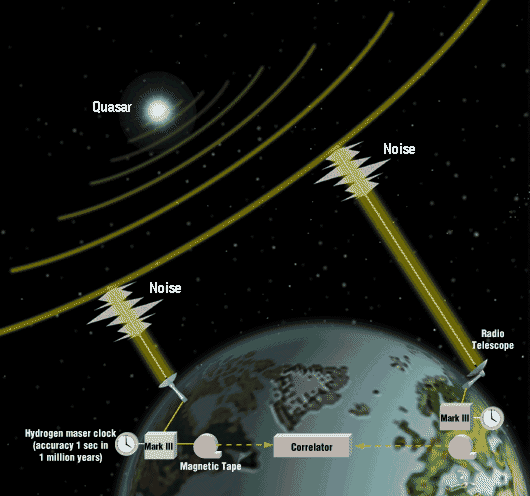
\includegraphics[width=\textwidth]{ch06/figures/vlbi.png}
\end{center}
\caption{In radio astronomy, the relative time delay between two Earth-based radio telescopes and a point like radio emission source is determining the rate of change of the relative phase as a function of frequency. Figure: NASA GFSC.}
\label{fig:vlbi_concept}
\end{marginfigure}

\section{Example: Very long baseline interferometry}
A point-like radio star emits a signal across a broad range of frequencies. This means that we can observe the signal originating from the radio star with multiple angular frequencies $\omega$. We can denote the signal originating from the star at a certain frequency with:
\begin{equation}
z(t,\omega) = A(\omega) e^{i\phi(\omega)} e^{i\omega t}
\end{equation}
Here $A(\omega) \in \mathbb{R}_{\ge 0}$ is the amplitude and $\phi(\omega)$ is the phase of the signal at angular frequency $\omega$. Because the signal is generated by an enormous collection of charged particles (primarily electrons) in an accelerating motion, the amplitudes and phases are random variables.

If we measure the signal originating from the radio star at two different places with a radio telescope simultaneously, the time of arrival of the signal between the two telescopes will differ by $\tau$ due to geometry (see Figure \ref{fig:vlbi_concept}). It is this value of $\tau$ that is often of interest, when, e.g., estimating the orientation of Earth relative to the stars. 

Let's denote the signal received with telescope 1 with $z_1$ and the signal received with telescope 2 with $z_2$:
\begin{align}
z_1(t,\omega) &= A(\omega) e^{i\phi(\omega)} e^{i\omega t} \\
z_2(t,\omega) &= A(\omega) e^{i\phi(\omega)} e^{i\omega (t-\tau)}
\end{align}
We'll assume that $z_1$ is the same signal as $z_2$, with only one exception, the signal $z_2$ is delayed by a time constant $\tau$ due to the receiver being further away 
from the source of the signal\sidenote{For radio signals, we need the radio source to be in the Fraunhofer far-field in order for this to be valid.}.

In order to determine the value $\tau$, we can use the following operation:
\begin{equation}
z_1(t,\omega)z_2^*(t,\omega) = |A(\omega)|^2 e^{i\omega \tau} 
\end{equation}
The random phase $\phi(\omega)$ cancels out with this operation, as well as the oscillating term $\omega t$. The phase of this cross-product only depends on frequency and time shift $\tau$:
\begin{equation}
\angle z_1(t,\omega)z_2^*(t,\omega) = \theta(\omega)= \omega \tau
\end{equation}
If we measure the cross-product $z_1(t,\omega)z_2^*(t,\omega)$ across a sufficiently wide range of frequencies, we can estimate $\tau$ using:
\begin{equation}
\frac{d\theta}{d\omega}= \tau
\end{equation}
This is a very simplified description of how the very long baseline interferometry technique used in radio astronomy and geodesy allows us to precisely measure the relative difference in time of arrival of a signal originating from a point-like radio source when measured with two different radio receivers.

\if 0
\section{Python example: plotting sinusoidal signals}

The following example will get you started with Python and signal
processing. It is a sort of a \index{Hello World}{Hello World}, which plots a sinusoid.
\begin{lstlisting}[language=Python]
import numpy as n
import matplotlib.pyplot as plt

# time vector (1000 samples per second) one second duration
t=n.arange(1000)/1000.0
# create a 10 Hz sinusoidal signal with amplitude 10
x=10.0*n.cos(2.0*n.pi*10.0*t)
# create a 10 Hz sinusoidal signal with amplitude 5, 
# time shifted by 0.02 s
xd=5.0*n.cos(2.0*n.pi*10.0*(t+0.02))

plt.plot(t,x,label="$x(2\pi 10 t)$")
plt.plot(t,xd,label="$x(2\pi 10(t+0.02))$")

plt.legend()
plt.show()
\end{lstlisting}
\fi

\section{Python example: shifting in frequency}

The following Python example demonstrates in practice
Equation \ref{eq:freqmix} which tells us that when multiplying two complex sinusoidal signals together, the resulting signal will have a frequency corresponding to the sum of the two frequencies of the multiplied signals.

\lstinputlisting[language=Python,caption={\texttt{005\_mixing/mixing.py}},label=lst:mixing_ex]{code/005_mixing/mixing.py}

\section{Example: Electromagnetic waves}
\label{waveeq}

This example will show that complex sinusoidal signals are a useful mathematical tool also for solving differential equations by deriving a plane wave solution of \index{electromagnetic waves}{electromagnetic waves} from \index{Maxwell's equations}{Maxwell's equations}.

Don't worry if you are not familiar with these equations. I mainly want you to pay attention to how the differential equation is solved for a plane wave using a \index{two-dimensional complex sinusoidal signal}{two-dimensional complex sinusoidal signal} $\vec{E}(x,t)=\hat{y}E_0 e^{i k x}e^{i\omega t}$. Because the exponential function is easy to differentiate, it is easy to apply this type of function for solving differential equations.

Assuming that there are no currents ($\vec{J}=0$) or space charges ($\rho=0$), \index{Maxwell's equations}{Maxwell's equations} are as follows:
\begin{align}
\nabla \cdot \vec{E} &= 0 \\
\nabla \cdot \vec{B} &= 0 \\
\nabla \cross \vec{E} &= -\frac{\partial \vec{B}}{\partial t} \label{eq:faraday}\\
\nabla \cross \vec{B} &= \epsilon_0 \mu_0 \frac{\partial \vec{E}}{\partial t} \label{eq:maxwell}
\end{align}
If we curl Faraday's law, we get:
\begin{align}
\nabla \cross (\nabla \cross \vec{E}) &= -\frac{\partial }{\partial t}\nabla \cross \vec{B}
\end{align}
If we then use the vector identity
$\nabla \cross (\nabla \cross \vec{E}) = \nabla(\nabla \cdot \vec{E}) - \nabla^2 \vec{E}$ and include Gauss' law for electric field $\nabla \cdot \vec{E} = 0$ in the case when there are no charges, we get
\begin{align}
\nabla^2 \vec{E} &= \frac{\partial }{\partial t}\nabla \cross \vec{B}
\end{align}
If we now insert the Maxwell–Ampere's law (Equation \ref{eq:maxwell}) into Faraday's
law (Equation \ref{eq:faraday}), we get:
\begin{align}
\frac{\partial^2 \vec{E}}{\partial t^2} - \frac{1}{\mu_0 \epsilon_0} \nabla^2 \vec{E} &= 0.
\end{align}
This type of equation is called a \index{wave equation}{wave equation}. You can also derive the same equation for the magnetic field, but we are not going to do that here.

Now let us assume that a solution to the wave equation is of the form:
\begin{equation}
\vec{E}(x,t)= E_0 \hat{y} e^{-i k x}e^{i\omega t}
\label{efieldplanewave}
\end{equation}
Here $E_0 \in \mathbb{C}$ is a complex number that determines the amplitude and phase of the electric field. The term $\hat{y}$ is a unit vector in the y-axis direction. 
In other words, a plane wave, where the electric field in the y-z plane is constant-valued. The electric field only changes as a function of position in the $x$-axis as a function of time $t$.

\begin{figure}
\begin{center}
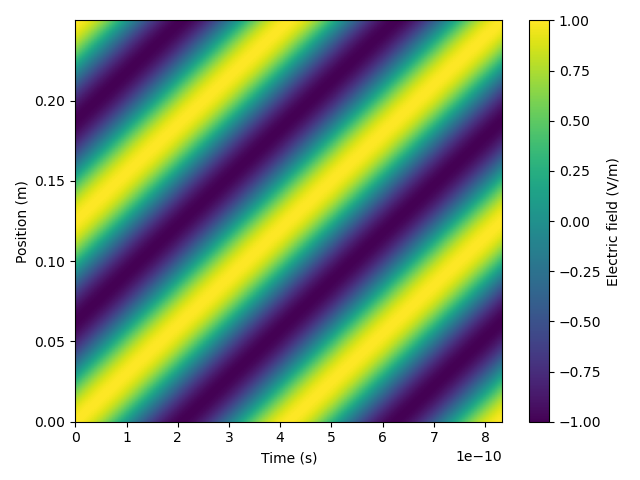
\includegraphics[width=\textwidth]{code/007_2dwave/em_plane_wave.png}
\end{center}
\caption{A plane wave solution to Maxwell's equations, describing propagation of electromagnetic waves in space and time. The script that produced this plot is \texttt{007\_2dwave/em\_plane\_wave.py}. }
\label{fig:planewave}
\end{figure}

It is easy to differentiate a complex exponential function twice in space and time. Remember that the \index{Laplacian operator}{Laplacian operator}, which is a linear system, is defined as:
\begin{equation}
\nabla^2 = \frac{\partial^2}{\partial x^2} + \frac{\partial^2}{\partial y^2} +\frac{\partial^2}{\partial z^2} 
\end{equation}
Because the electric field is constant in the y-z plane, only the second derivative in the x-direction remains. Using the two-dimensional plane wave formulation of Equation \ref{efieldplanewave}, we can see that
\begin{align}
\frac{\partial ^2 \vec{E}}{\partial t^2} &= -\omega^2 \vec{E}(x,t) \\
\nabla^2 \vec{E} &= -k^2 \vec{E}(x,t).
\end{align}
And therefore, the wave equation becomes:
\begin{align}
\frac{\partial^2 \vec{E}}{\partial t^2} - \frac{1}{\mu_0 \epsilon_0} \nabla^2 \vec{E} &= 0 \\
(c^2k^2-\omega^2) \vec{E}(x,t) &= 0 \label{eq:disp_relation}
\end{align}
I've taken the liberty of changing the constant $c = (\mu_0\epsilon_0)^{-1/2}$ for reasons that will become apparent soon. 
The constant $\mu_0$ is permeability of free space, and $\epsilon_0$ is permittivity of free space. The value of $c \approx 3\cdot 10^{8}$ m/s.

In order for the two-dimensional complex sinusoidal signal to be consistent with Maxwell's equations, either $E(x,t)=0$ or $c^2k^2-\omega^2 = 0$. 
The trivial solution $E(x,t)=0$ is not very interesting, as there would be no electric field. The latter describes a solution with a non-zero electric field, as long as the following relationship:
\begin{equation}
k = \pm \frac{\omega}{c}
\end{equation}
is satisfied. This means that the following two-dimensional signal is a solution to the Maxwell's equations:
\begin{align}
\vec{E}(x,t) &= E_0 \hat{y} e^{-i (\omega/c) x} e^{i\omega t} \\
             &= E_0 \hat{y} e^{-i 2\pi \lambda^{-1} x} e^{i 2\pi f t} 
\end{align}
Here, I've used the relation $2\pi f = \omega$. I've also used the wavelength of the electromagnetic wave, which is $\lambda = c/f$. 
In other words, we have used a two-dimensional complex sinusoidal signal and the Maxwell's equations to describe how electromagnetic waves propagate in space and time.

I am showing the real part of the plane wave solution in
Figure \ref{fig:planewave}. In this case, the frequency is chosen to
be $f=2.4$ GHz, which is the frequency typically used by microwave
ovens and wireless internet (which you are probably using right
now). Try to figure out what is the velocity that a region of constant
phase propagates in the positive x-axis direction at.



